\documentclass[crop,class=article]{standalone}
%----------------------------Preamble-------------------------------%
\usepackage{tikz}                       % Drawing/graphing tools.
%--------------------------Main Document----------------------------%
\begin{document}
    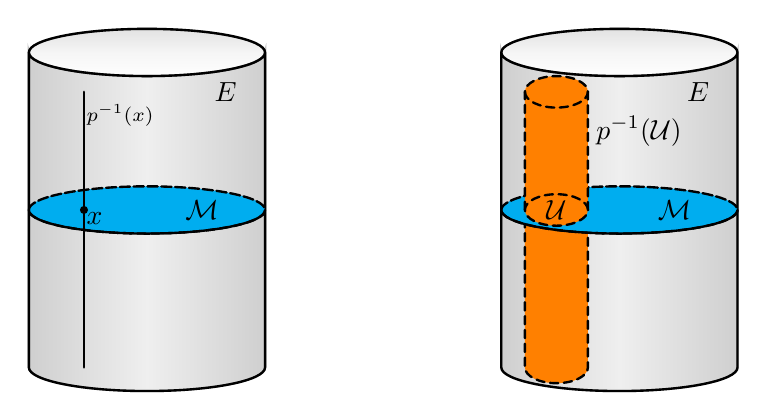
\begin{tikzpicture}[%
        line width=0.3mm,
        line cap=round,
    ]
        \draw[%
            left color=gray!50!black,
            right color=gray!50!black,
            middle color=gray!50,
            shading=axis,
            opacity=0.25
        ]   (1.5,0) to (1.5,4) arc (360:180:1.5cm and 0.3cm)
                    to (-1.5,0) arc (180:360:1.5cm and 0.3cm);
        \draw[%
            top color=gray!90!,
            bottom color=gray!2,
            middle color=gray!30,
            shading=axis,
            opacity=0.25
        ]   (0,4) circle (1.5cm and 0.3cm);
        \draw (-1.5,4) to (-1.5,0) arc (180:360:1.5cm and 0.3cm)
                       to (1.5,4) (0,4) circle (1.5cm and 0.3cm);
        \draw[fill=cyan,densely dashed]
            (-1.5,2) arc (180:0:1.5cm and 0.3cm) 
                     arc (360:0:1.5cm and 0.3cm);
        \draw (-1.5,2) arc (180:360:1.5cm and 0.3cm);
        \node[%
            circle,
            fill=black,
            draw=black,
            inner sep=0pt,
            minimum size=2pt
        ]   at (-0.8,2) {};
        \node at (-0.9,2.1) [below right] {$x$};
        \node at (0.7,2) {$\mathcal{M}$};
        \node at (1,3.5) {$E$};
        \node at (-0.9,3.2) [right] {\scriptsize{$p^{-1}(x)$}};
        \draw (-0.8,0) to (-0.8,3.5);

        % Shift for the second cylinder.
        \begin{scope}[xshift=6cm]
            \draw[%
                left color=gray!50!black,
                right color=gray!50!black,
                middle color=gray!50,
                shading=axis,
                opacity=0.25
            ]   (1.5,0) to (1.5,4) arc (360:180:1.5cm and 0.3cm)
                        to (-1.5,0) arc (180:360:1.5cm and 0.3cm);
            \draw[%
                top color=gray!90!,
                bottom color=gray!2,
                middle color=gray!30,
                shading=axis,
                opacity=0.25
            ]   (0,4) circle (1.5cm and 0.3cm);
            \draw (-1.5,4) to (-1.5,0) arc (180:360:1.5cm and 0.3cm)
                           to (1.5,4) (0,4) circle (1.5cm and 0.3cm);
            \draw[densely dashed, fill=orange]
                (-0.4,2) to (-0.4,0) arc (360:180:4mm and 2mm)
                         to (-1.2,2);
            \draw[fill=cyan,densely dashed]
                (-1.5,2) arc (180:0:1.5cm and 0.3cm) 
                         arc (360:0:1.5cm and 0.3cm);
            \draw (-1.5,2) arc (180:360:1.5cm and 0.3cm);
            \draw[densely dashed, fill=orange]
                (-1.2,2) to (-1.2,3.5) arc (180:0:4mm and 2mm)
                         to (-0.4,2);
            \draw[densely dashed,fill=orange]
                (-0.8,2) circle (4mm and 2mm);
            \draw[densely dashed]
                (-1.2,3.5) arc (180:360:4mm and 2mm);
            \node at (-0.8,2) {$\mathcal{U}$};
            \node at (0.7,2) {$\mathcal{M}$};
            \node at (1,3.5) {$E$};
            \node at (0.25,3) {$p^{-1}(\mathcal{U})$};
        \end{scope}
    \end{tikzpicture}
\end{document}